\documentclass[
	%sans,			% use sans-serif font
	%serif,			% use serif-font
	%mathsans,		% set mathtext to sans-serif
	%mathserif,		% set mathtext to serif
	%10pt,
	10pt,
	%12pt,
	t		% add text at the top border of slide
	%slidescentered,% center text on slide
	%draft,			% compile as draft version
	%handout,		% create handout file
	%notes,			% include nodes in slides
	%compress		% compress navigation bar
]{beamer}

\usetheme{lmtslides}
\usepackage{eso-pic}
\usepackage{graphicx}
%\usepackage[pdftex]{color}
\usepackage{times}
\usepackage[latin1]{inputenc}
%\usepackage[T1]{fontenc}
\usepackage[amssymb]{SIunits}
\usepackage{amsmath,amssymb}
\usepackage{eurosym}
\usepackage{booktabs}
\usepackage{colortbl}
\usepackage{url}
\usepackage[absolute,overlay]{textpos}
\usepackage{graphicx}
\usepackage{mathtools}
\usepackage{pifont}% http://ctan.org/pkg/pifont

\newcommand{\xmark}{\ding{55}}%
\newcommand{\cmark}{\ding{51}}%

\renewcommand{\footnoterule}{\vfill\kern -3pt  \kern 2.6pt}

\setbeamertemplate{caption}{\raggedright\insertcaption\par}
\setbeamertemplate{bibliography item}[online]
\graphicspath{{figures/}}

\setlang{en}		

% Supervisor: Univ.-Prof. Dr. Hans-Joachim Bungartz
% Advisors: Manish Kumar Mishra, M.Sc. (hons) &
% Samuel James Newcome, M.Sc.

% MODIFY THESE ACCORDINGLY! ---
\title{Exploring Fuzzy Tuning Technique for Molecular Dynamics Simulations in AutoPas}
\type{Bf} % (M/B/D/S)(f/m): (Master/Bachelor/Diplom/Studienarbeit)(final/midterm)
\author{Manuel Lerchner}
\email{manuel.lerchner@tum.de}
\advisorOne{Manish Kumar Mishra, M.Sc.}
\advisorTwo{Samuel James Newcome, M.Sc.}
\date{\today}
%------------------------------


%%%%%%%%%%%%%%%%%%%%%%%%%%
\begin{document}

\maketitle

\setcounter{framenumber}{0}

\section{Introduction}
\begin{frame}
	\frametitle{What is AutoPas?}
	
	\begin{textblock*}{5cm}(9cm,1.8cm)
		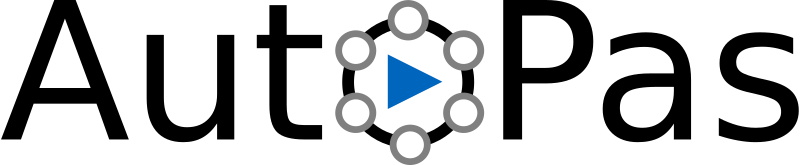
\includegraphics[width=3cm]{figures/AutoPasLogo}
	\end{textblock*}
	
	\begin{itemize}
		\item Library for arbitrary N-body simulations
		\item Optimal performance by switching implementations
		      \begin{itemize}
			      \item \textbf{Container:} Finding neighboring particles
			      \item \textbf{Traversal:} Parallel force calculations
			      \item \textbf{Data Layout:} Memory access optimization
			      \item \textbf{Newton 3:} Force calculation optimization
		      \end{itemize}
	\end{itemize}
	
	\vspace{-0.1cm}
	\begin{figure}
		\centering
		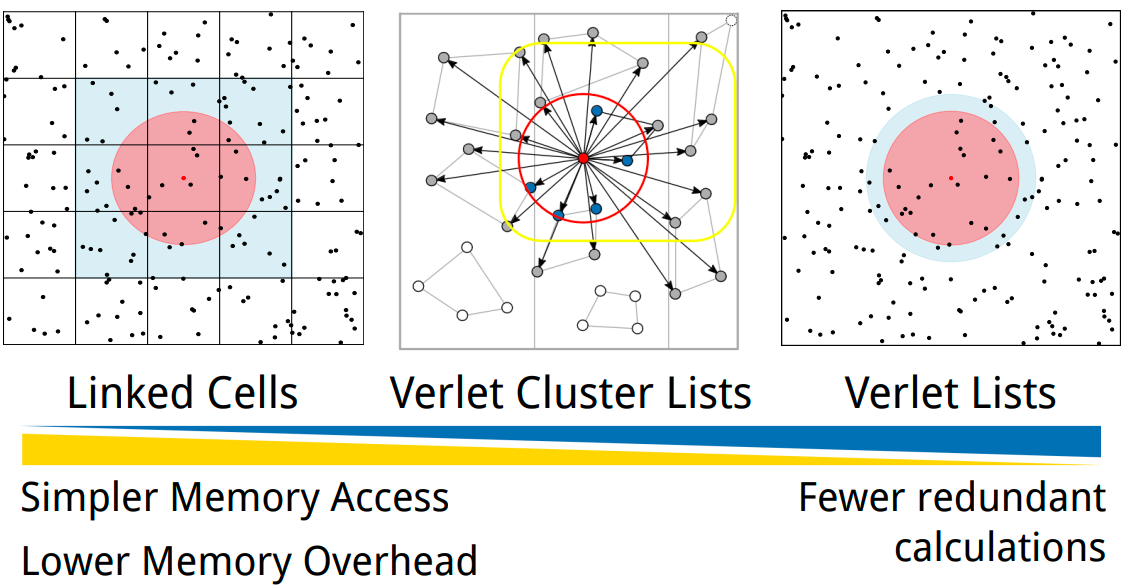
\includegraphics[width=0.72\textwidth]{figures/traversals.png}
	\end{figure}
	
	\begin{textblock*}{5cm}(6.3cm,9.35cm)
		\tiny{\cite{SIAM_PP24}}
	\end{textblock*}
	
\end{frame}


\begin{frame}
	\frametitle{Structure of AutoPas}
	
	\begin{itemize}
		\item Three main areas:
		      \begin{itemize}
			      \item User Application
			      \item Algorithm Library
			      \item Tuning Strategies
		      \end{itemize}
		\item Algorithm Library:
		      \begin{itemize}
			      \item Huge Search Space\footnote{\scriptsize{$\text{Container}\times\text{Traversal} \times \text{Data Layout} \times \text{Newton 3} \times \text{Load Estimator} \times \text{Cell Size Factor}$}
			            }
		      \end{itemize}
		\item Tuning Strategies:
		      \begin{itemize}
			      \item Full Search
			      \item Random Search
			      \item Predictive Tuning
			      \item Bayesian Search
			      \item Rule Based Tuning
		      \end{itemize}
	\end{itemize}
	
	\begin{textblock*}{4cm}(8cm,2cm)
		\begin{figure}
			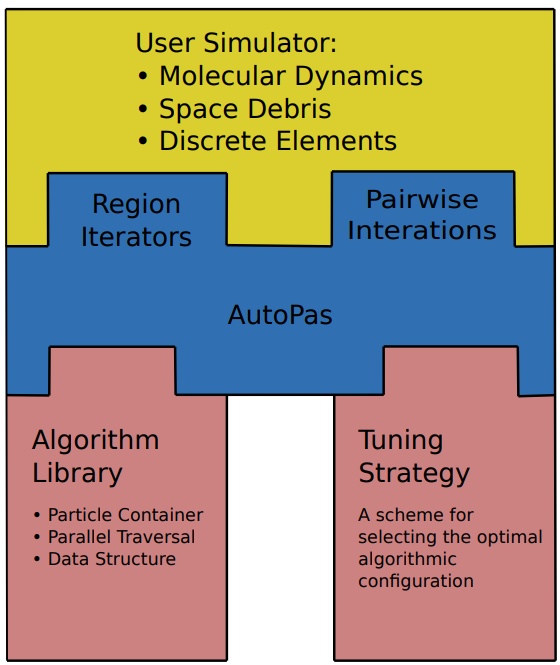
\includegraphics[width=4cm]{figures/AutoPasLibraryStructure.png}
			\caption{ \footnotesize{Source: \cite{Newcome2023Poster}}}
			
		\end{figure}
	\end{textblock*}
\end{frame}



\begin{frame}
	\frametitle{Auto-Tuning }
	
	\begin{itemize}
		\item Tuning Phase $\rightarrow$ Simulation Phase $\rightarrow$ Repeat
		\item Potential Tuning Overhead
	\end{itemize}
	
	\vspace{0.1cm}
	
	\begin{figure}
		\makebox[\textwidth][c]{
			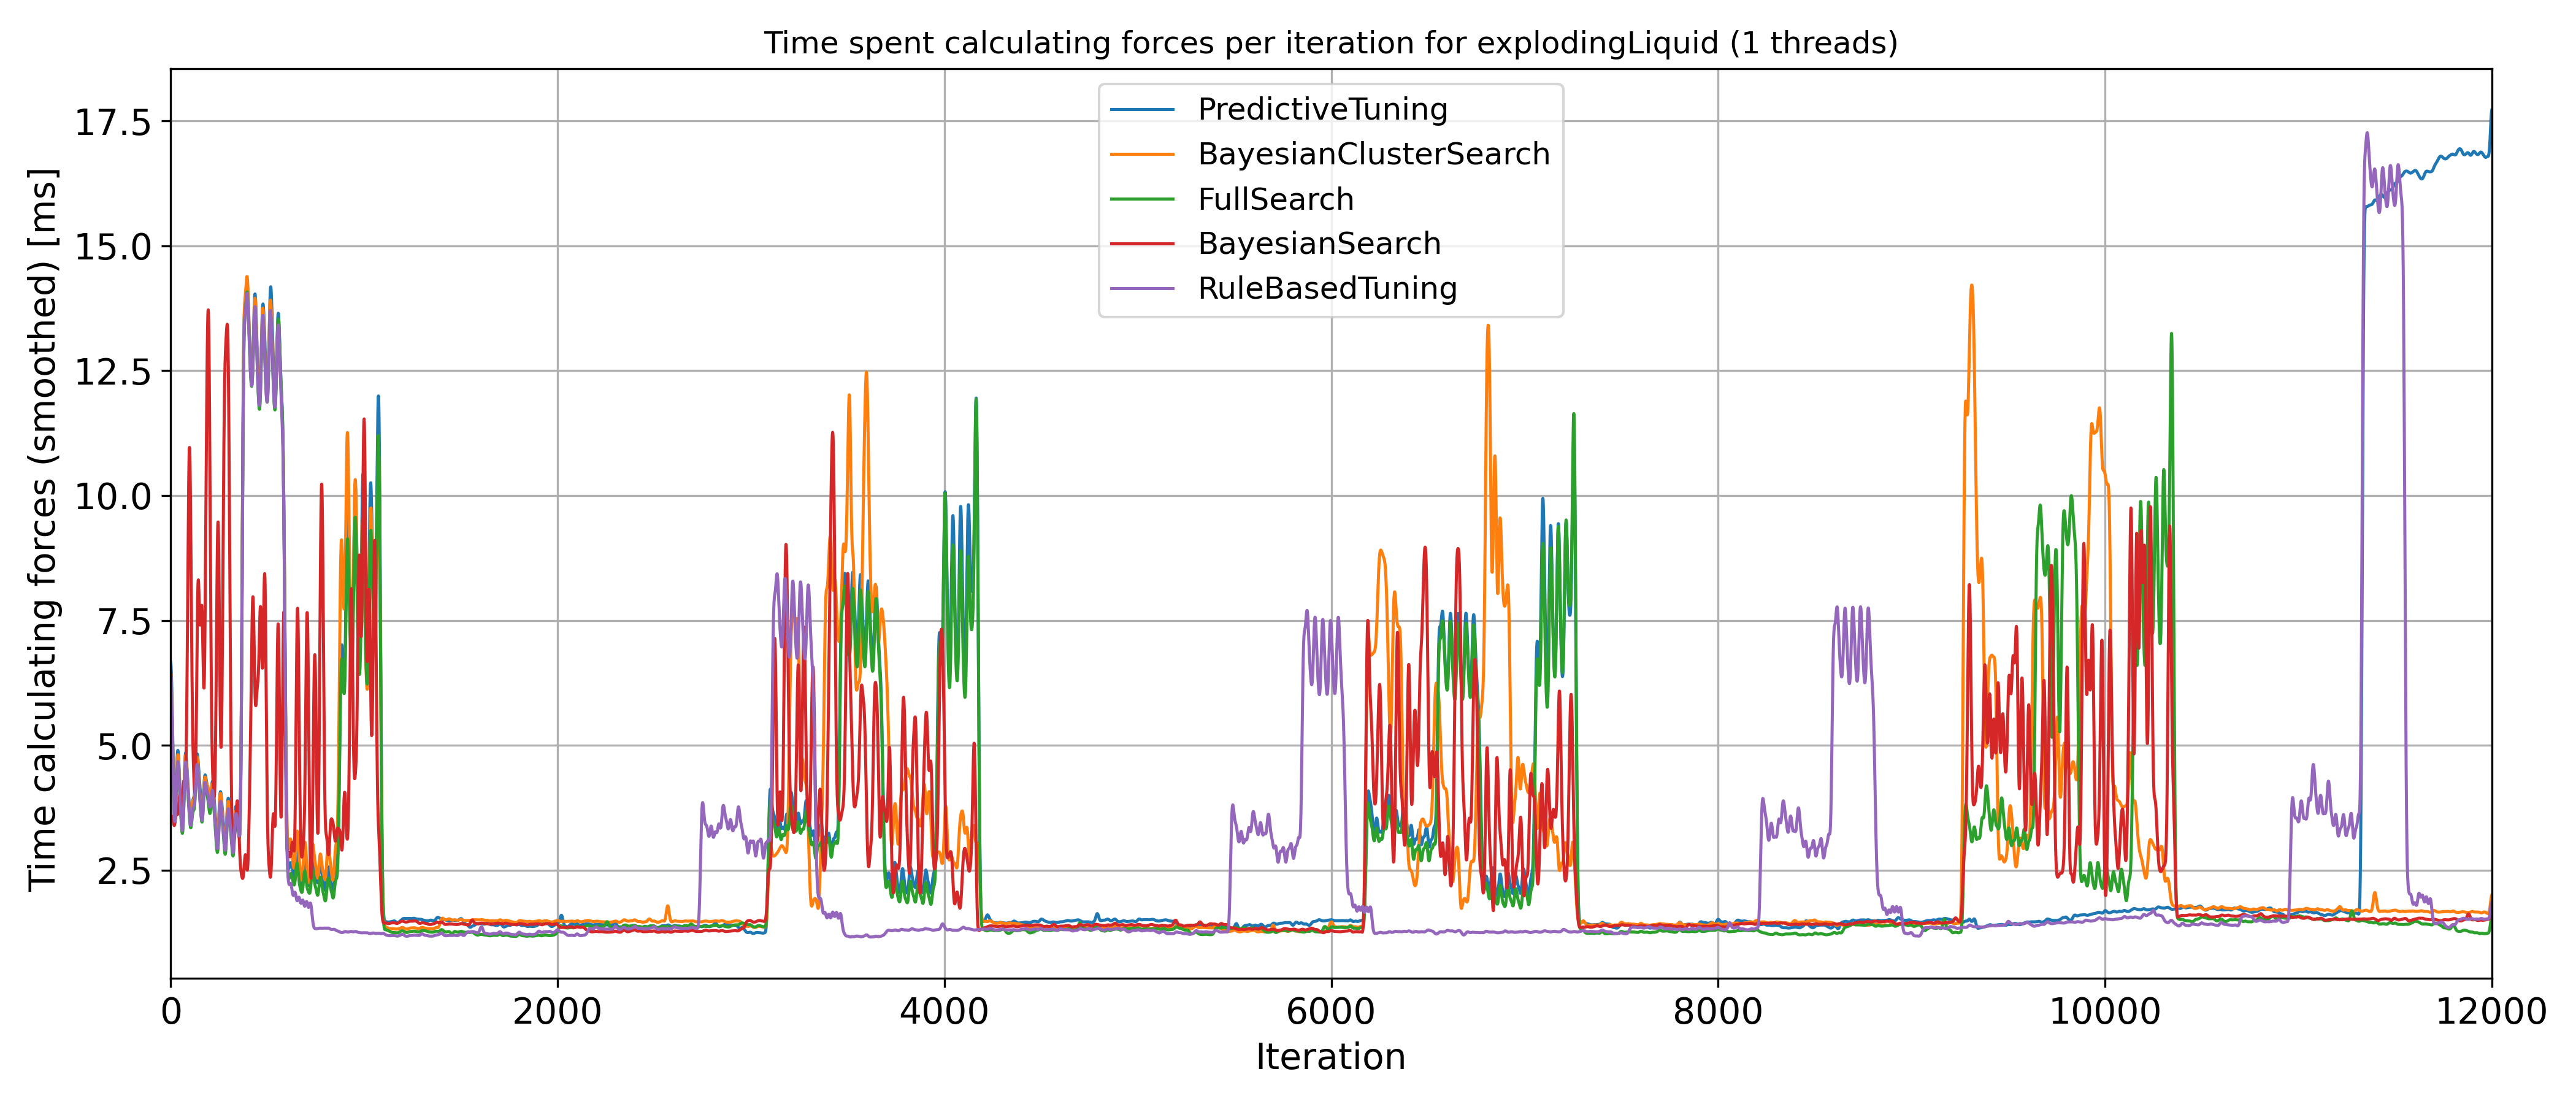
\includegraphics[width=1.1\textwidth,trim={0 0 0 0.85cm},clip]{figures/timing_explodingLiquid.png}
		}
	\end{figure}
	
	
\end{frame}

\begin{frame}
	\frametitle{Fuzzy Logic Systems}
	
	\begin{itemize}
		\item Human-like reasoning to model systems $f: \mathbb{R}^n \rightarrow \mathbb{R}$
		\item (Fuzzy) Rule based systems
		      \begin{itemize}
			      \item Interpolation effect between conflicting rules
			      \item No hard boundaries $\rightarrow$ robust against noise
		      \end{itemize}
		\item Smooth transition instead of hard boundaries
		      \begin{itemize}
			      \item E.g. \textit{cold, warm, hot} instead of \textit{20$^{\circ}$C, 30$^{\circ}$C, 40$^{\circ}$C}
		      \end{itemize}
	\end{itemize}
	
	\vspace{0.4cm}
	
	\begin{example}[Heater Control]
		
		\begin{description}[wide=0]
			\item[\textbf{Input:}  ] ~ temperature (e.g. 20$^{\circ}$C), humidity (e.g. 60\%)
			\item[\textbf{Output:}] heater power (e.g. 50\%)
			\item[\textbf{Rules:}]
				{\footnotesize
				\begin{tabular}{lcll}
					\textbf{IF}  temp is \textit{cold} & \textbf{AND} & humidity is \textit{dry} & \textbf{THEN}  power is \textit{high}   \\
					\textbf{IF}  temp is \textit{hot}  & \textbf{OR}  & humidity is \textit{wet} & \textbf{THEN}  power is \textit{low}    \\
					\textbf{IF}  temp is \textit{warm} &              &                          & \textbf{THEN}  power is \textit{medium} \\
				\end{tabular} }
		\end{description}
	\end{example}
	
\end{frame}

% \begin{frame}
% 	\frametitle{Naming Conventions}

% 	\begin{itemize}
% 		\item Consider the Fuzzy Rule:
% 		      \[
% 			      \underbrace{  \underbrace{\textbf{IF}  \;\underbrace{\text{temp}}_{\text{Ling. Var.}} \text{is} \underbrace{\textit{cold}}_{\text{Ling. Term}}  \textbf{AND}  \underbrace{\text{hum}}_{\text{Ling. Var.}} \text{is} \underbrace{\textit{dry}}_{\text{Ling. Term}} }_{\text{Antecedent}}
% 				      \textbf{THEN}  \underbrace{\underbrace{\text{power}}_{\text{Ling. Var.}} \text{is} \underbrace{\textit{high}}_{\text{Ling. Term}}}_{\text{Consequent}}
% 			      }_{\text{Fuzzy Rule}}
% 		      \]
% 		\item Fuzzy Logic Systems consist of:
% 		      \begin{itemize}
% 			      \item Linguistic Terms / Fuzzy Sets (e.g. \textit{cold, warm, hot})
% 			      \item Linguistic Variables (e.g. temperature, humidity, power)
% 			      \item Fuzzy Logic Operators (e.g. \textbf{AND, OR, NOT})
% 			      \item Fuzzy Rules (e.g. \textbf{IF} \textit{antecedent} \textbf{THEN} \textit{consequent})
% 		      \end{itemize}
% 	\end{itemize}
% \end{frame}

% \begin{frame}
% 	\frametitle{Fuzzy Sets vs Classical Sets}
% 	\begin{itemize}
% 		\item Fuzzy Sets are generalizations of classical sets
% 		      \begin{itemize}
% 			      \item $U$ is the universe of discourse (e.g. $age \subseteq \mathbb{R}$)
% 			      \item Classical Set $A \subseteq U$:
% 			            \begin{itemize}
% 				            \item Defined via indicator function $\chi_A : U \rightarrow \{0,1\}$
% 			            \end{itemize}
% 			      \item Fuzzy Sets $\tilde{A} \subseteq U$:
% 			            \begin{itemize}
% 				            \item Defined via \textbf{Continuous} membership function $\mu_{\tilde{A}} : U  \rightarrow [0,1]$
% 			            \end{itemize}
% 		      \end{itemize}
% 	\end{itemize}
% 	\begin{center}
% 		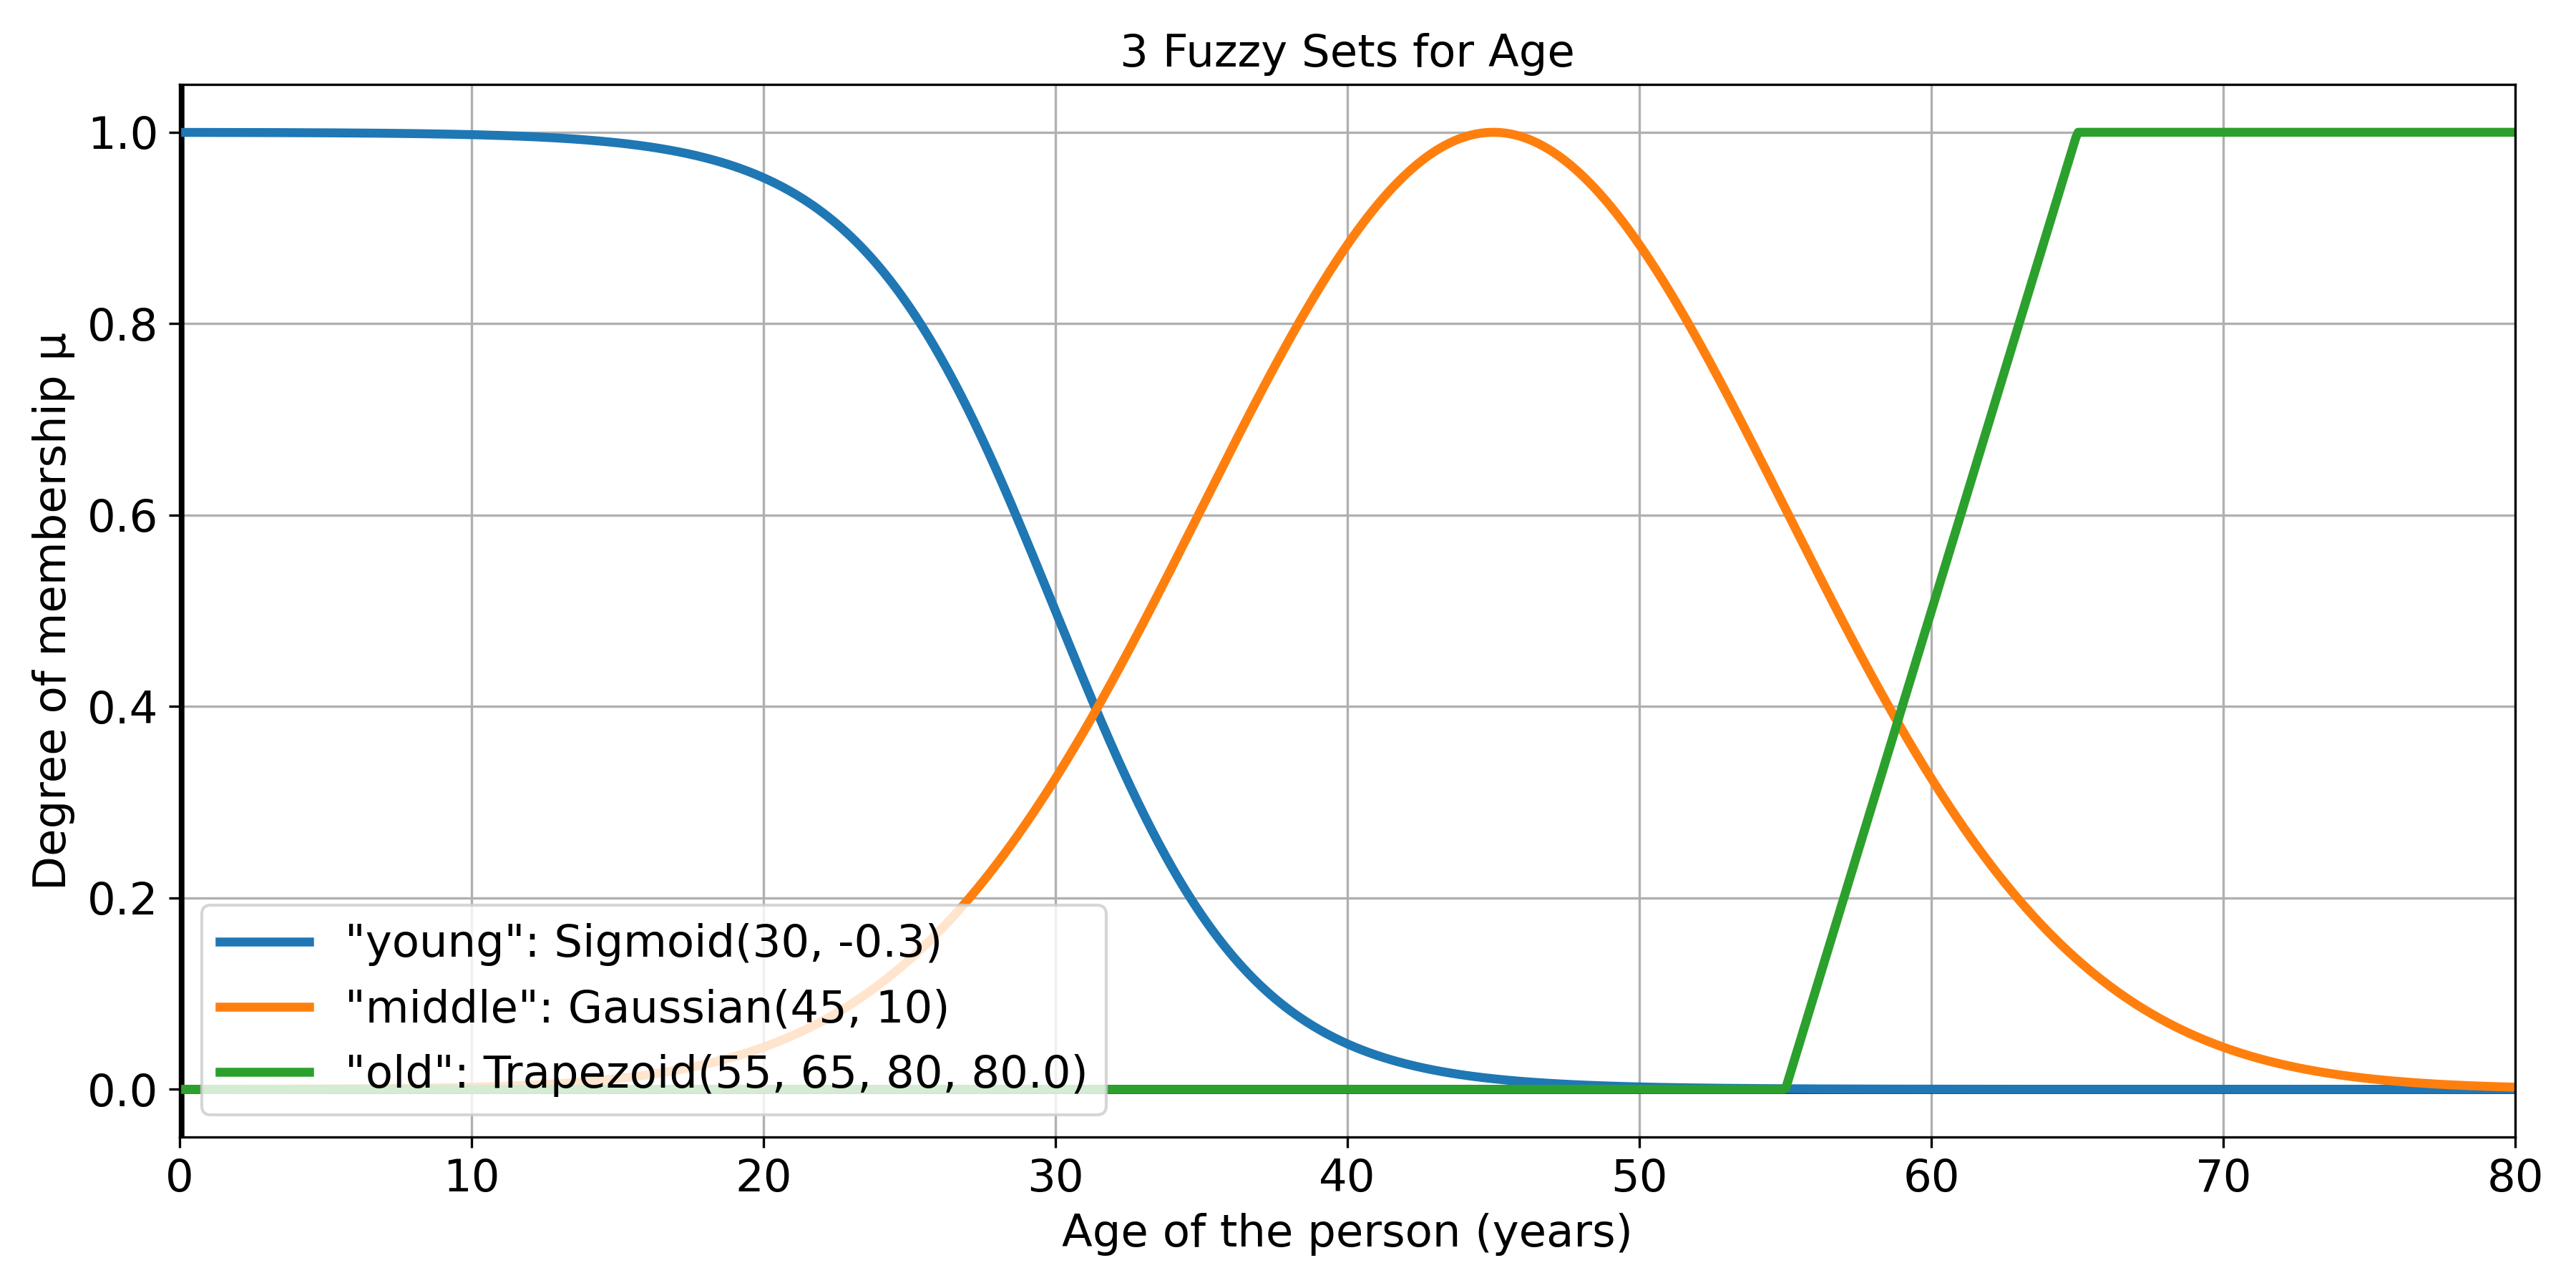
\includegraphics[width=0.8\textwidth,trim={0 0.1cm 0 1.2cm},clip]{figures/age-fuzzy-sets.png}
% 	\end{center}
% \end{frame}

% \begin{frame}
% 	\frametitle{Linguistic Variables}
% 	\begin{itemize}
% 		\item Use terms instead of numeric values
% 		\item Instead of using crisp values (35 years), we use a combination of linguistic terms to describe the age (Fuzzyification):
% 		      \[ \text{ 35 years} \implies  \begin{cases}
% 				      \text{20\% young}       \\
% 				      \text{60\% middle-aged} \\
% 				      \text{0\% old}
% 			      \end{cases}
% 		      \]
% 		\item This allows for non-numerical reasoning:
% 		      \begin{itemize}
% 			      \item E.g. \textbf{IF} age is \textit{young} \textbf{THEN} fitness is \textit{high}
% 			      \item Use abstract concepts instead of crisp values
% 		      \end{itemize}
% 		\item Each linguistic term represents a certain \textit{collection} of values with varying degrees of membership
% 	\end{itemize}
% \end{frame}

% \begin{frame}
% 	\frametitle{Fuzzy Logic Operators}
% 	\begin{itemize}
% 		\item Fuzzy Logic Operators are used to modify/combine fuzzy sets
% 		\item Extension of boolean logic operators to real numbers
% 		      \begin{itemize}
% 			      \item $\wedge : \{false, true\} \times \{false, true\} \rightarrow \{false, true\}$
% 			      \item $\textbf{AND} : [0,1] \times [0,1] \rightarrow [0,1]$
% 		      \end{itemize}
% 		\item Fuzzy operators defined via extension of set
% 		      \begin{itemize}
% 			      \item Need to maintain the classical semantics
% 			      \item Boolean logic is a special case of fuzzy logic
% 		      \end{itemize}

% 		\item Typically, Fuzzy Logic Operators are defined as:
% 		      \begin{itemize}
% 			      \item \textbf{AND:} Corresponds to the intersection of fuzzy sets
% 			            \[ \mu_{\tilde{A} \cap \tilde{B}}(x) = \min(\mu_{\tilde{A}}(x), \mu_{\tilde{B}}(x)) \]
% 			      \item \textbf{OR:} Corresponds to the union of fuzzy sets
% 			            \[ \mu_{\tilde{A} \cup \tilde{B}}(x) = \max(\mu_{\tilde{A}}(x), \mu_{\tilde{B}}(x)) \]
% 			      \item \textbf{NOT:} Corresponds to the complement of a fuzzy set
% 			            \[ \mu_{\neg \tilde{A}}(x) = 1 - \mu_{\tilde{A}}(x) \]

% 		      \end{itemize}
% 	\end{itemize}
% \end{frame}

% \begin{frame}
% 	\vspace{0cm}
% 	\begin{figure}
% 		\centering
% 		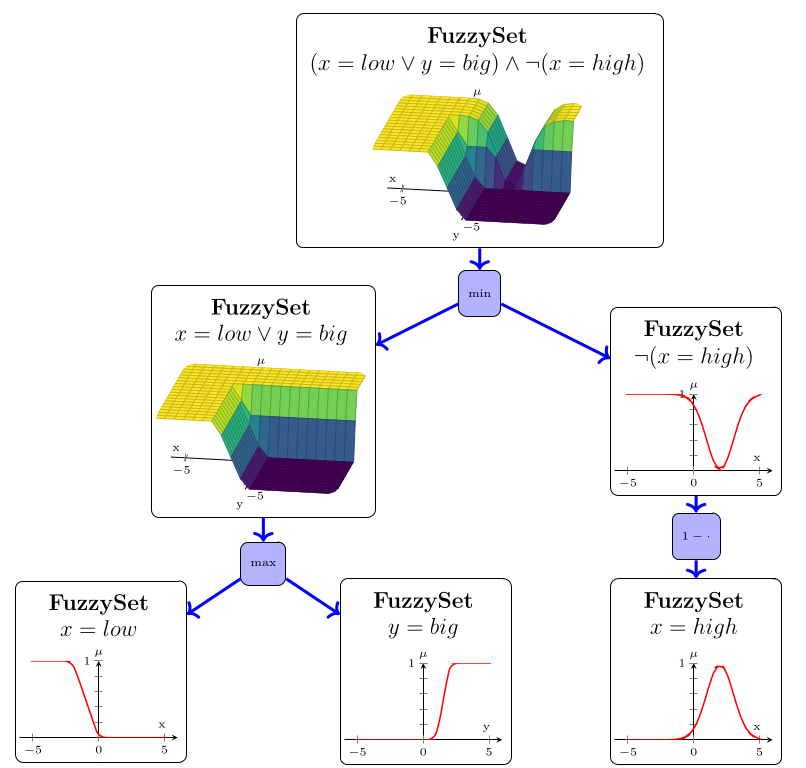
\includegraphics[height=0.62\paperwidth]{figures/RecursiveFuzzyTree.png}
% 	\end{figure}
% \end{frame}

% \begin{frame}
% 	\frametitle{Fuzzy Rules}
% 	\begin{itemize}
% 		\item Each rule is of the form: $\textbf{IF} \; {antecedent} \; \textbf{THEN} \; {consequent}$
% 		      \begin{itemize}
% 			      \item Both \textit{antecedent} and \textit{consequent} are fuzzy sets
% 			      \item E.g. $\textbf{IF} \; \text{age} \; \text{is} \; \textit{young} \; \textbf{THEN} \; \text{fitness} \; \text{is} \; \textit{high}$
% 		      \end{itemize}
% 		\item Rules are evaluated as logical implications
% 		      \begin{itemize}
% 			      \item $\textbf{IF} \; \tilde{A} \; \textbf{THEN} \; \tilde{B} \quad \iff \quad \tilde{A} \;  \textbf{IMPLIES} \;  \tilde{B}$
% 			      \item Special form of (fuzzy) implication: Mamdani Implication
% 			            \begin{itemize}
% 				            \item $\tilde{R} = \textbf{IF} \; \tilde{A} \; \textbf{THEN} \; \tilde{B}$
% 				            \item $\mu_{\tilde{R}}(x) = \min(\mu_{\tilde{A}}(x), \mu_{\tilde{B}}(x))$
% 			            \end{itemize}
% 			      \item \textit{Effect} of the rule is limited by the \textit{strength} of the antecedent
% 		      \end{itemize}
% 		\item Multiple rules can act on the same linguistic variable
% 		      \begin{itemize}
% 			      \item The total \textit{effect} on the output is the aggregation/union of all individual fuzzy sets
% 			      \item Each rule \textit{effect} is considered proportional to the \textit{strength} of its antecedent
% 		      \end{itemize}
% 	\end{itemize}
% \end{frame}

% \begin{frame}
% 	\frametitle{Defuzzification}
% 	\begin{itemize}
% 		\item Process of converting arbitrary fuzzy sets to a crisp value
% 		      \begin{itemize}
% 			      \item Special case: Fuzzy sets corresponding to a fuzzification
% 			            \[  \begin{cases}
% 					            \text{20\% young}       \\
% 					            \text{60\% middle-aged} \\
% 					            \text{0\% old}
% 				            \end{cases} \implies \text{35 years}
% 			            \]
% 		      \end{itemize}
% 		\item Multiple methods for defuzzification:
% 		      \begin{itemize}
% 			      \item \textbf{Center of Gravity:} Considers all values based on their membership. Finds weighted average of all possible values
% 			      \item \textbf{Mean of Maxima:} Considers only the most likely values (with highest membership). Finds the mean of all maxima
% 		      \end{itemize}
% 		\item Core idea: Represent aspects of the fuzzy set with a crisp value
% 		      \begin{itemize}
% 			      \item E.g. Weighted average of all possible values (Centroid)
% 			      \item E.g. Most likely value (Mean of Maxima)
% 		      \end{itemize}
% 	\end{itemize}

% \end{frame}



\begin{frame}
	\vspace{-0.8cm}
	\begin{figure}
		\centering
		\caption{\tiny{Source: \href{https://de.mathworks.com/help/fuzzy/fuzzy-inference-process.html}{MathWorks - Fuzzy Inference Process}}}
		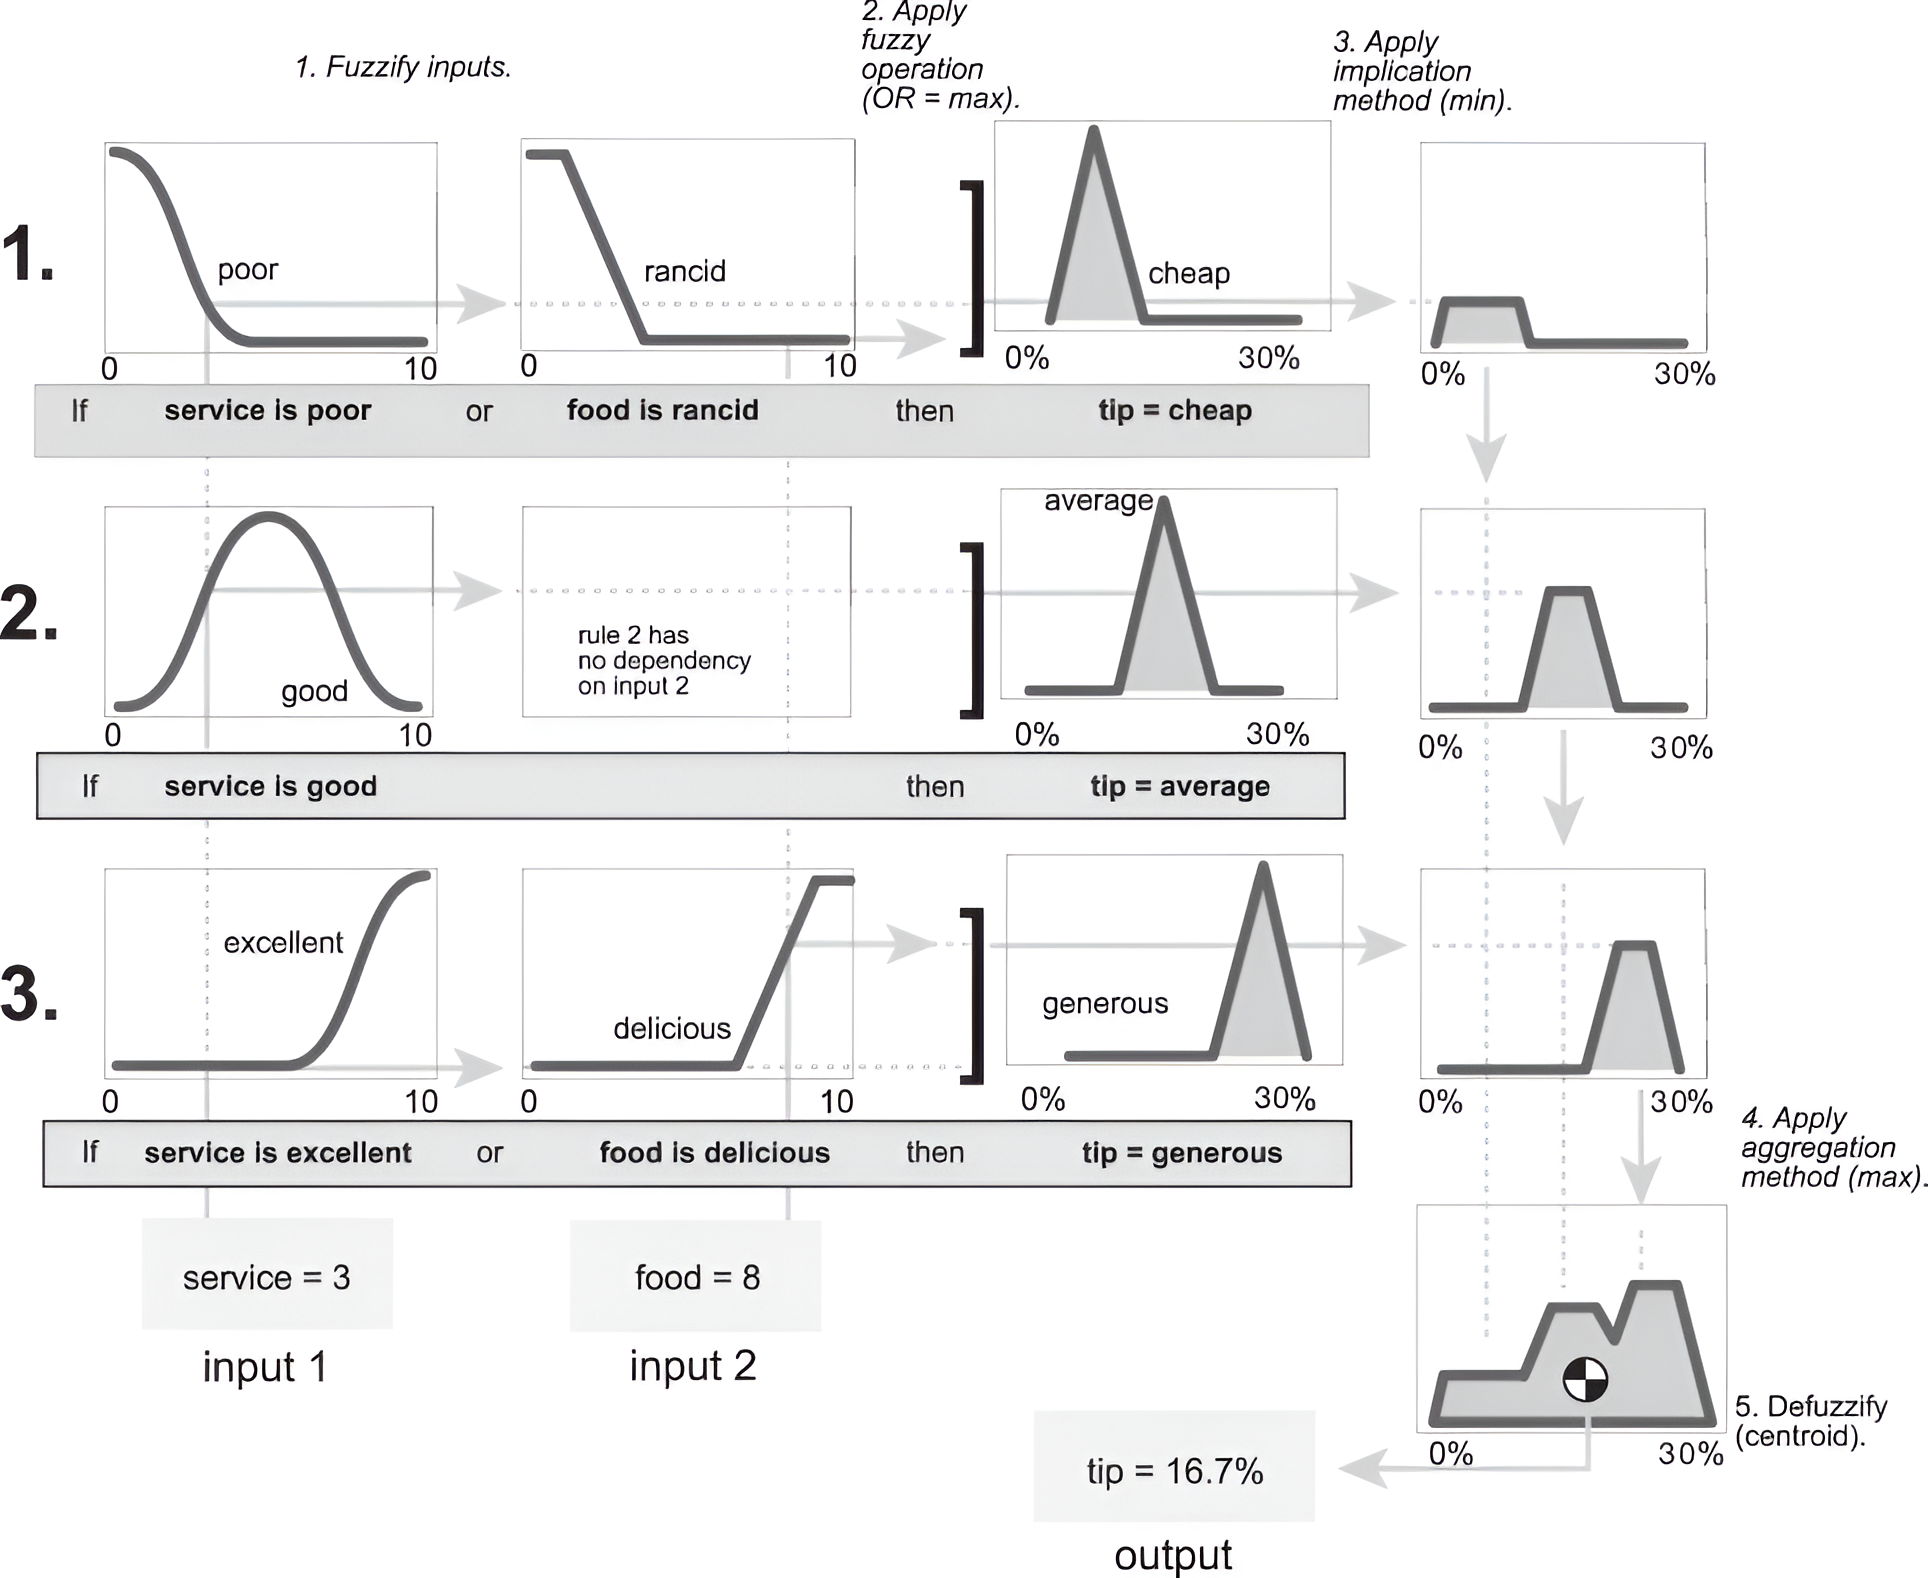
\includegraphics[width=0.8\paperwidth]{figures/FullInferenceProcess.png}
	\end{figure}
	\label{fig:fuzzy_inference_full}
	
\end{frame}


\section{Fuzzy Tuning Implementation}
\begin{frame}
	\frametitle{Fuzzy Tuning for AutoPas}
	
	\begin{itemize}
		\item Main Idea: Use Fuzzy Logic to tune AutoPas
		\item Expected Benefits:
		      \begin{itemize}
			      \item Expert knowledge allows efficient tuning phases\\
			            \quad \cmark \; Minimal tuning overhead \\
			            \quad \cmark \; Allows frequent tuning phases
			      \item Comes with \textit{interpolation} effect\\
			            \quad \cmark \; Fewer rules than Rule-Based tuning \\
			            \quad \cmark \; Generalization to new environments
			      \item Simplicity of the model\\
			            \quad \cmark \; Easy to understand and interpret\\
			            \quad \cmark \; Easy to maintain
		      \end{itemize}
	\end{itemize}
\end{frame}

\section{Fuzzy Tuning Implementation}
\begin{frame}
	\frametitle{Challenges and Questions}
	
	\begin{itemize}
		\item Fuzzy Tuning not directly applicable to AutoPas
		      \begin{itemize}
			      \item Tuning is an \textit{algorithm selection} problem
			      \item Fuzzy tuning provides functions $f :\mathbb{R}^n \rightarrow \mathbb{R}$
			      \item Big Question: How to interpret the numerical output?\\
			            \quad $\rightarrow$ \textit{Component Tuning} Approach \\
			            \quad $\rightarrow$ \textit{Suitability Tuning} Approach
		      \end{itemize}
		\item How to design the Fuzzy System?
		      \begin{itemize}
			      \item Creating it manually?\\
			            \quad \xmark \; Requires extensive expert knowledge\\
			            \quad \xmark \; Difficult to formalize non-trivial knowledge
			      \item Extracting rules from data?\\
			            \quad \cmark \; No prior expert knowledge required\\
			            \quad \cmark \; Semi-automated process\\
			            \quad \cmark \; Good starting point for human tuning
		      \end{itemize}
	\end{itemize}
\end{frame}

\begin{frame}
	\frametitle{Approach 1: Component Tuning}
	\begin{itemize}
		\item Predict good values for each tunable parameter separately
		\item Explicit Fuzzy System for each tunable parameter
		      \begin{itemize}
			      \item Output Variable: Continuous representation of the parameter
			      \item \textit{Discrete} implementations are placed in the output space
			      \item Map numerical output to the \textit{closest} value\\
			            \quad {\footnotesize (Inspired by: \cite{Mohammed2022})}
		      \end{itemize}
		\item Combine individual predictions to form final configuration(s)
	\end{itemize}
	
	\begin{figure}
		\centering
		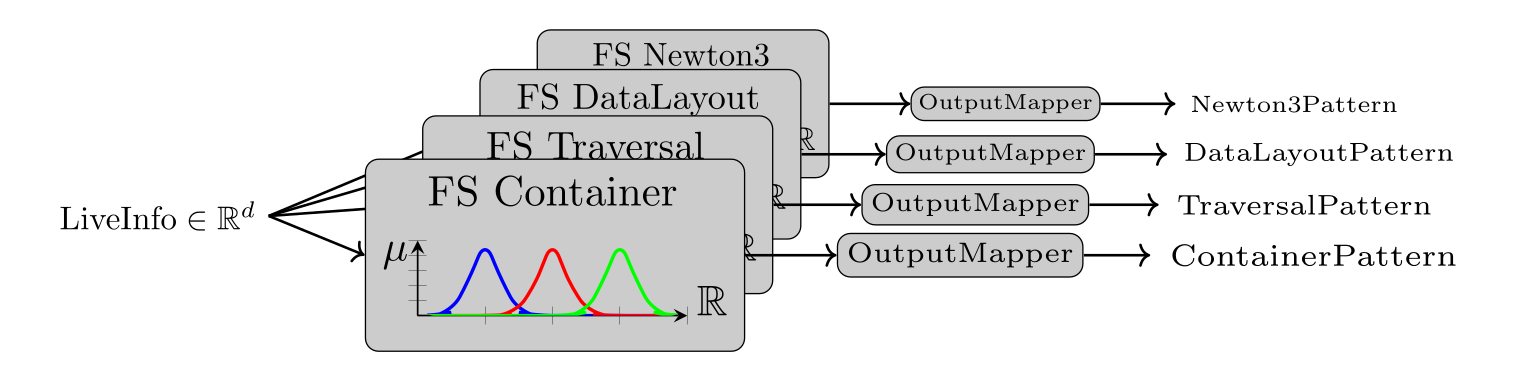
\includegraphics[width=1\textwidth]{figures/component-approach.png}
	\end{figure}
	
\end{frame}

\begin{frame}
	\frametitle{Approach 1: Component Tuning (Example)}
	\begin{itemize}
		\item Style: {\small \textbf{IF} avgParticlesPerCell is \textit{low} \textbf{AND} threadCount is \textit{low}\\ \qquad  \qquad \quad \textbf{THEN} traversal is \textit{vcl\_c06}}
		\item \textbf{Benefits:}
		      \begin{itemize}
			      \item Few fuzzy systems
			      \item Few and natural rules
		      \end{itemize}
		\item \textbf{Drawbacks:}
		      \begin{itemize}
			      \item Limited interpolation effect (MoM defuzzification)
			      \item Independence assumption
		      \end{itemize}
		      
		      
	\end{itemize}
	
	\begin{figure}
		\centering
		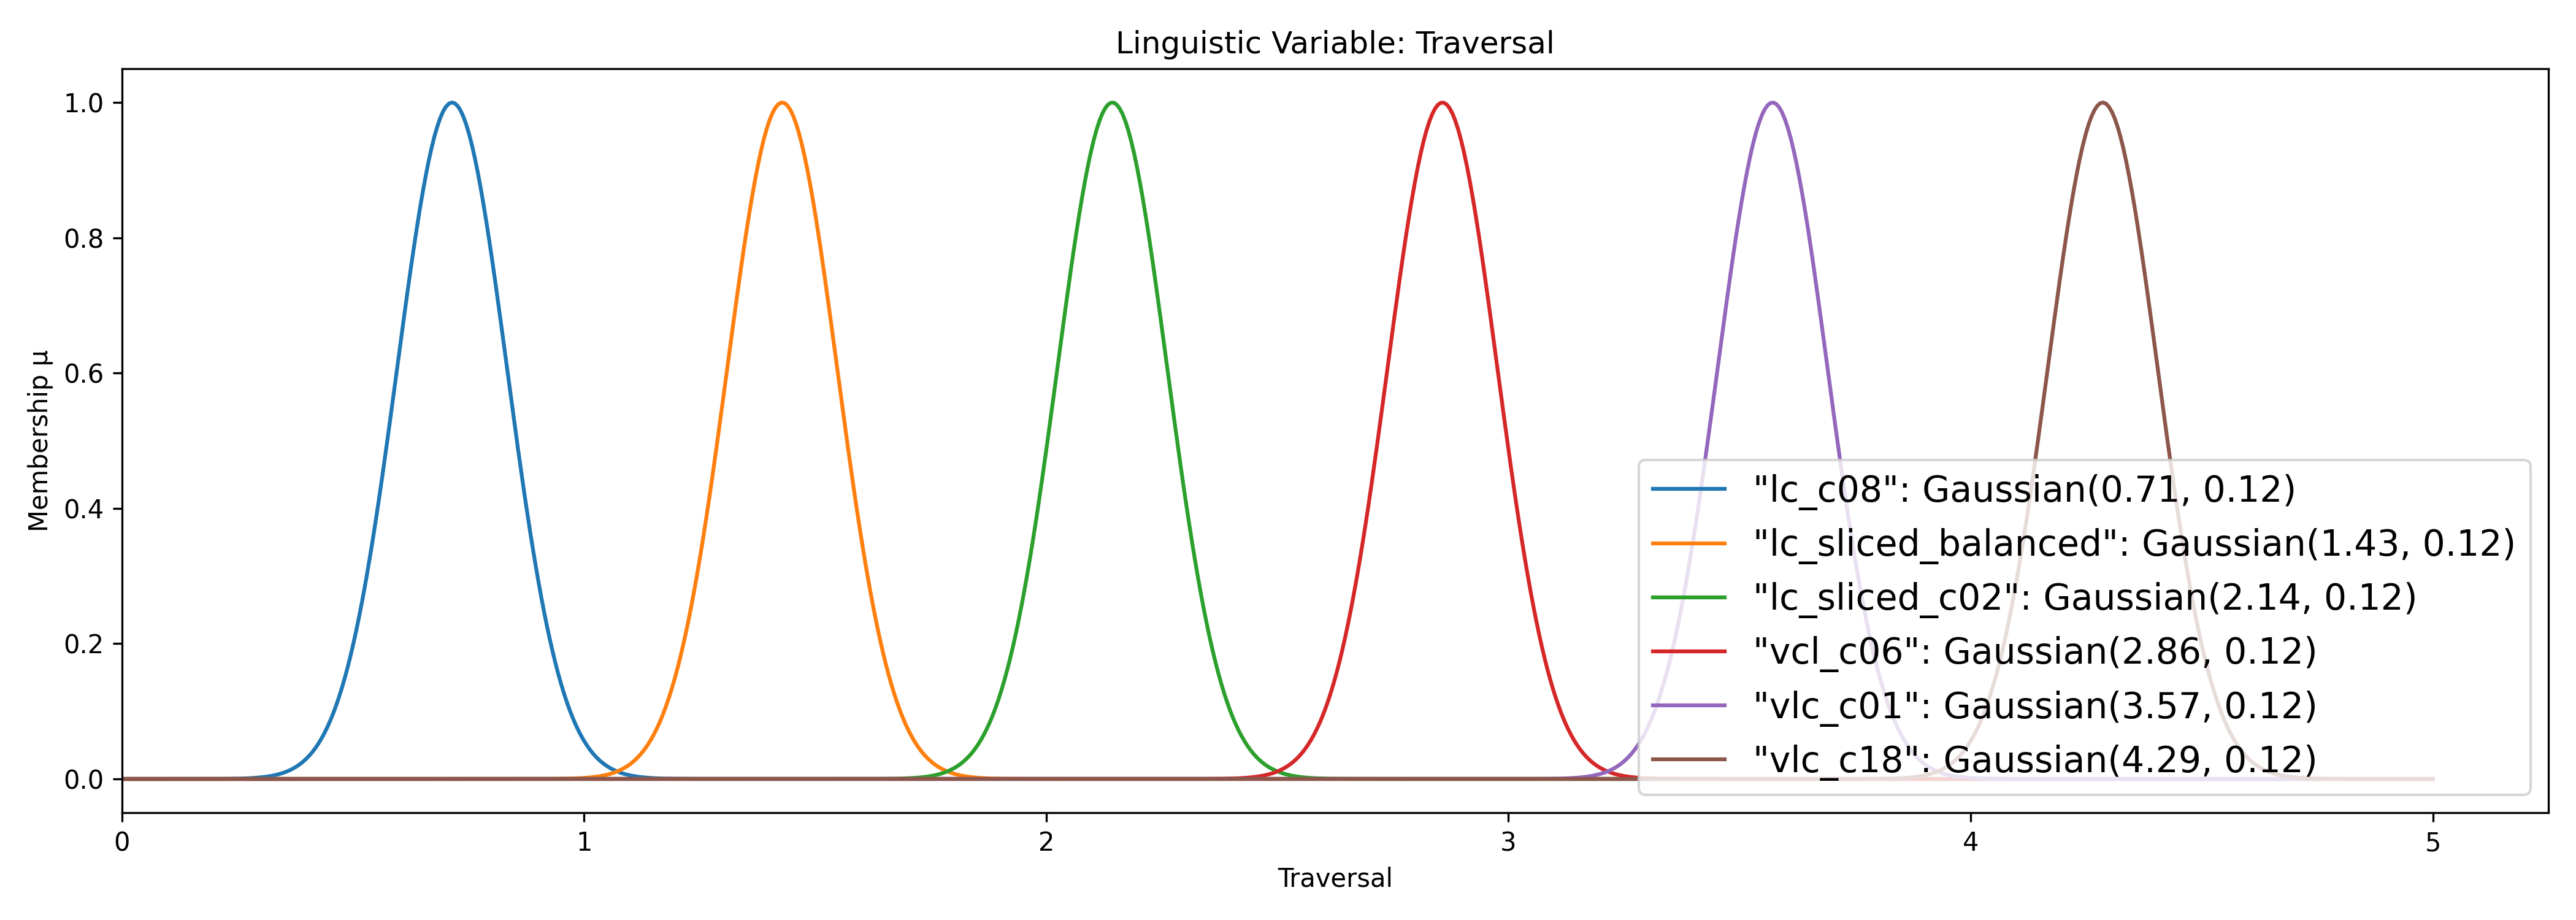
\includegraphics[width=0.9\textwidth,trim={0 0 0 1cm},clip]
		{figures/component-linguistic-variable.png}
	\end{figure}
	
\end{frame}



\begin{frame}
	\frametitle{Approach 2: Suitability Tuning}
	\begin{itemize}
		\item Predict the $suitability$ of \textbf{each} configuration separately
		\item Explicit Fuzzy System for all possible configurations
		      \begin{itemize}
			      \item Output Variable: Numerical suitability of the configuration
		      \end{itemize}
		\item Results in $(suitability, configuration)$ pairs
		      \begin{itemize}
			      \item \textit{Best} configurations are selected
		      \end{itemize}
	\end{itemize}
	
	\begin{figure}
		\centering
		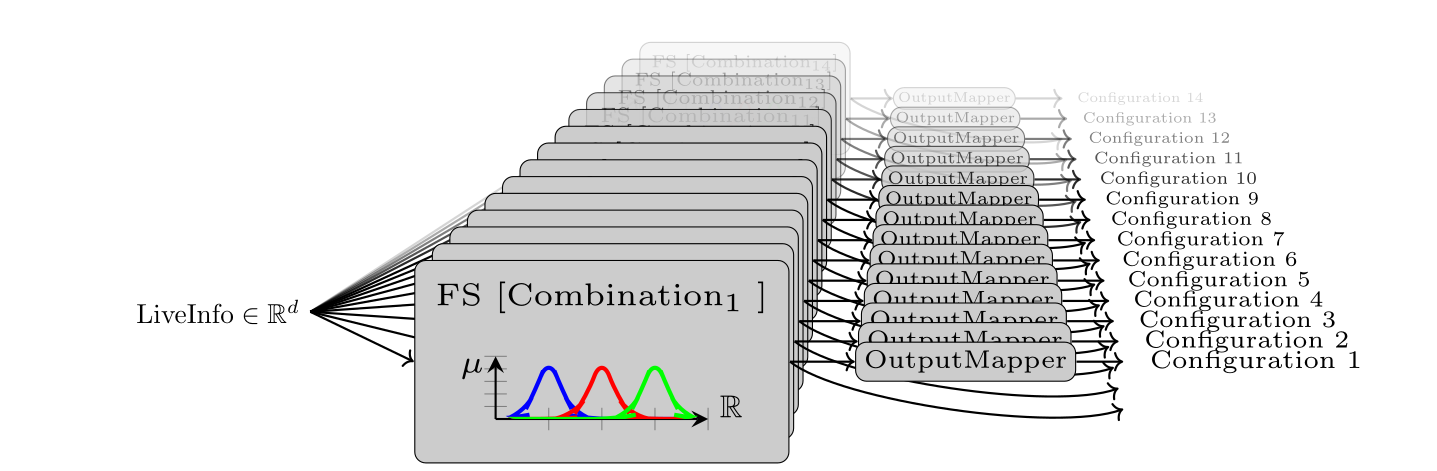
\includegraphics[width=1\textwidth]{figures/suitability-approach.png}
	\end{figure}
\end{frame}


\begin{frame}
	\frametitle{Approach 2: Suitability Tuning (Example)}
	\begin{itemize}
		\item Style: {\small
		      \textbf{IF} threadCount is \textit{high} \textbf{AND} avgParticlesPerCell is \textit{low}\\ \qquad \qquad \quad \textbf{THEN} suitability\_LinkedCells\_AoS\_lc\_c18\_disabled is \textit{bad}}
		      
		\item \textbf{Benefits:}
		      \begin{itemize}
			      \item Utilizes the full power of fuzzy logic (CoG defuzzification)
			      \item Dependencies and incompatibilities can be modeled
		      \end{itemize}
		\item \textbf{Drawbacks:}
		      \begin{itemize}
			      \item Huge number of fuzzy systems
			      \item Impossible to maintain by hand
		      \end{itemize}
	\end{itemize}
	
	\begin{figure}
		\centering
		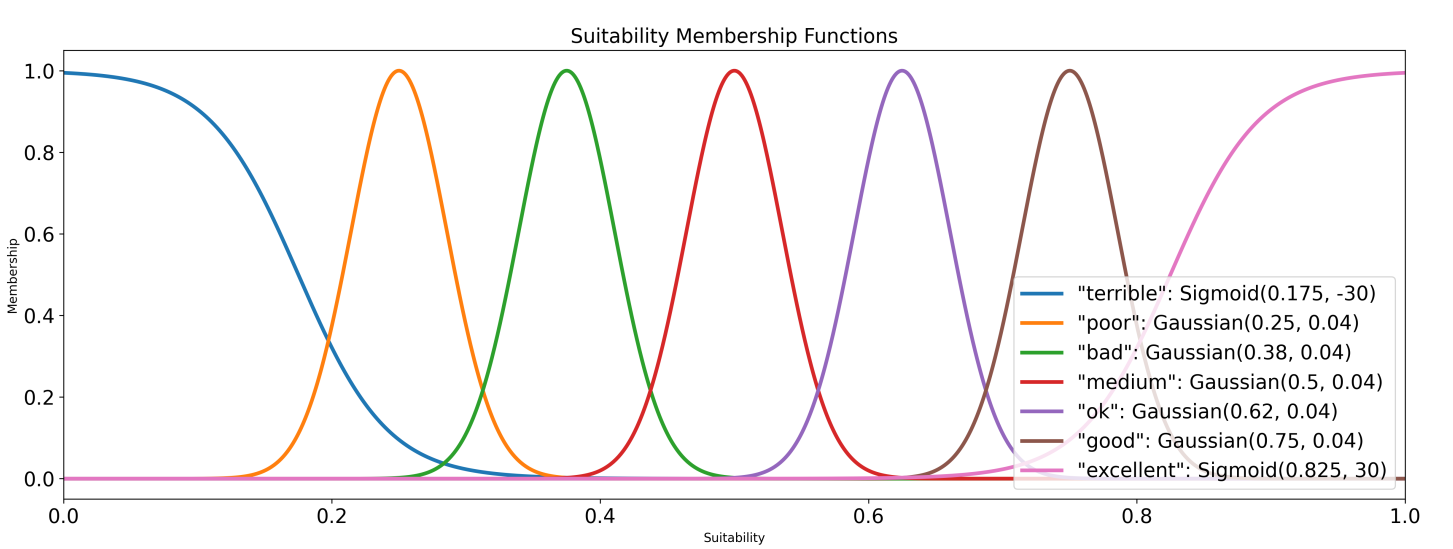
\includegraphics[width=0.82\textwidth,trim={0 0 0 1.8cm},clip]{figures/suitability-linguistic-variable.png}
	\end{figure}
	
\end{frame}


\begin{frame}
	\frametitle{Data-Driven Rule Extraction}
	\begin{itemize}

		\item Use data to automatically generate fuzzy systems
		      \begin{itemize}
			      \item Utilize machine learning techniques to extract rules
			      \item We follow \cite{CROCKETT20062809}
			            \begin{enumerate}
				            \item Train a Decision Tree on the data
				            \item Decision Tree $\rightarrow$ Fuzzy Decision Tree
				            \item Fuzzy Decision Tree $\rightarrow$ Fuzzy Rules
			            \end{enumerate}
		      \end{itemize}
		\item Practical Considerations:
		      \begin{itemize}
			      \item Ensemble Learning for Decision Trees
			            \begin{itemize}
				            \item Train with selected features
				            \item Different splitting criteria
				            \item Different tree depths / pruning
			            \end{itemize}
			      \item \textit{Overlapping} rules $\rightarrow$ \textit{Interpolation} effect
		      \end{itemize}
	\end{itemize}
\end{frame}

\begin{frame}
	\frametitle{Decision Trees}
	
	\begin{itemize}
		\item Seperate classes recursively with axis-aligned splits
		\item Corresponds to nested \textit{if-then-else} rules
		      \begin{itemize}
			      \item Easy to understand and interpret
		      \end{itemize}
		\item Trained automatically from data
		\item Tree contains the entire expert knowledge
	\end{itemize}
	
	\begin{figure}
		\centering
		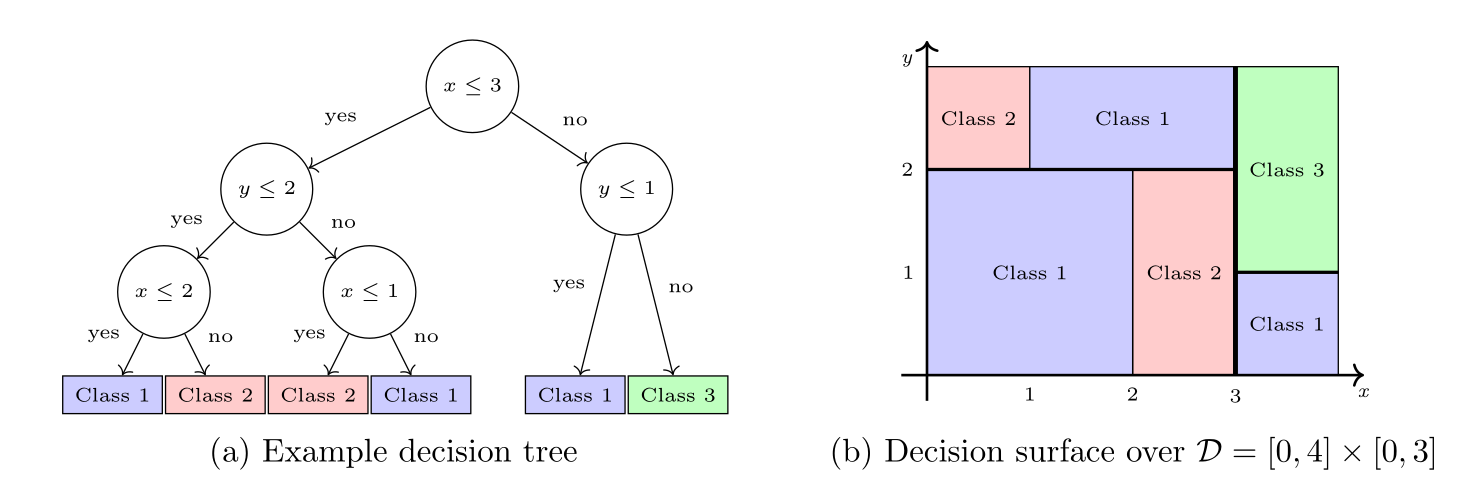
\includegraphics[width=1\textwidth]{figures/decision-tree.png}
	\end{figure}
	
\end{frame}

\begin{frame}
	\frametitle{Decision Trees $\rightarrow$ Fuzzy Decision Trees}
	
	\begin{itemize}
		\item Conversion: Each (crisp) split is turned into two fuzzy sets
		      \begin{itemize}
			      \item Fuzzy sets should maintain the semantics of the split
			      \item Provides robustness against noise
		      \end{itemize}
		\item Leaf nodes are turned into fuzzy sets
		      \begin{itemize}
			      \item Each class corresponds to a fuzzy set
		      \end{itemize}
	\end{itemize}
	\begin{figure}
		\centering
		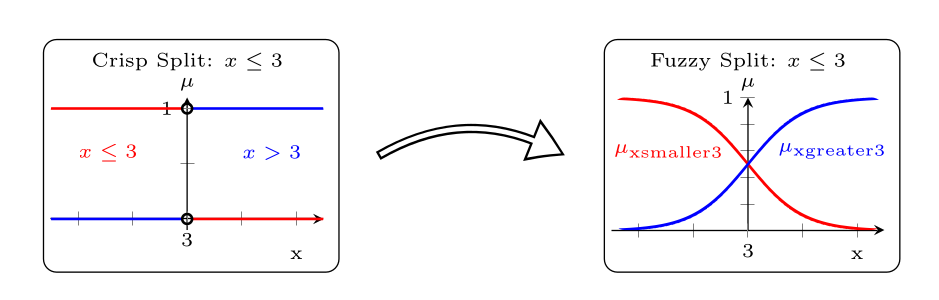
\includegraphics[width=8cm]{figures/leaf-conversion.png}
	\end{figure}
	
\end{frame}

\begin{frame}

	\begin{figure}
		\centering
		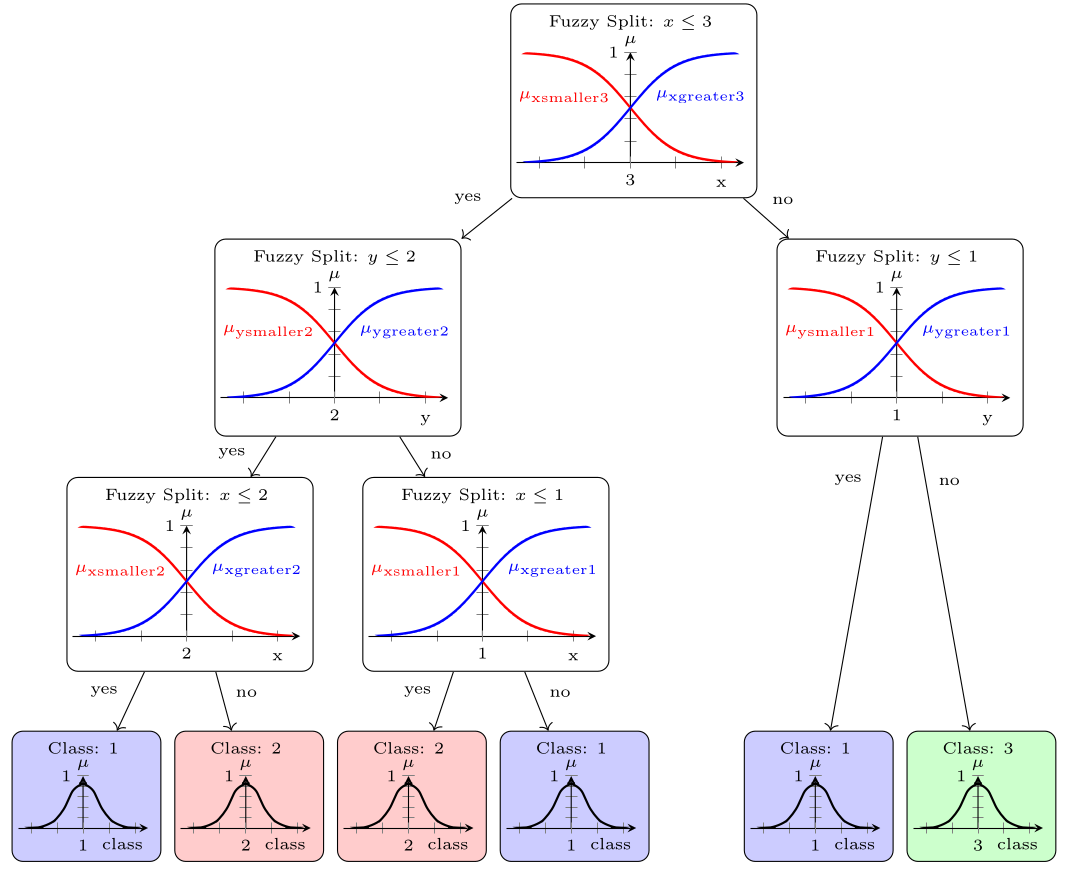
\includegraphics[width=0.9\textwidth]{figures/fuzzy-decision-tree.png}
	\end{figure}
	
\end{frame}

\begin{frame}

	\frametitle{Fuzzy Decision Trees $\rightarrow$ Fuzzy Rules}
	
	\begin{itemize}
		\item Depth-First traversal of the Fuzzy Decision Tree
		      \begin{itemize}
			      \item Fuzzy splits are collected in the antecedent
			      \item Leaf node corresponds to the consequent
		      \end{itemize}
		\item One rule per path from root to leaf
		\item Corresponds to \textit{unnesting} the decision tree
	\end{itemize}
	
	\begin{figure}
		\centering
		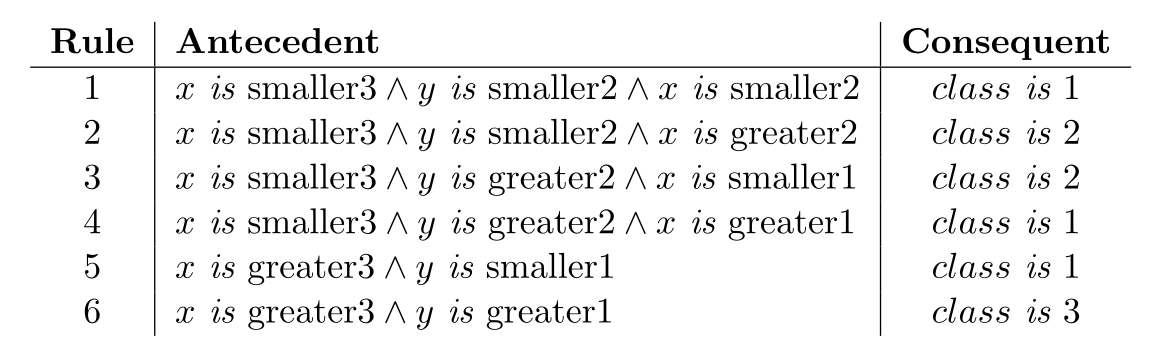
\includegraphics[width=0.9\textwidth]{figures/extracted-rules.png}
	\end{figure}
	
\end{frame}

\begin{frame}

	\frametitle{Decision Surfaces}
	
	\begin{itemize}
		\item Defuzzification Method affects the decision surface
		      \begin{itemize}
			      \item CoG: Interpolation effect, smooth boundaries
			      \item MoM: Most likely class, hard boundaries
		      \end{itemize}
		\item CoG: \textit{Interpolation errors} for nominal values
	\end{itemize}
	
	\vspace{-0.2cm}
	
	\begin{figure}
		\centering
		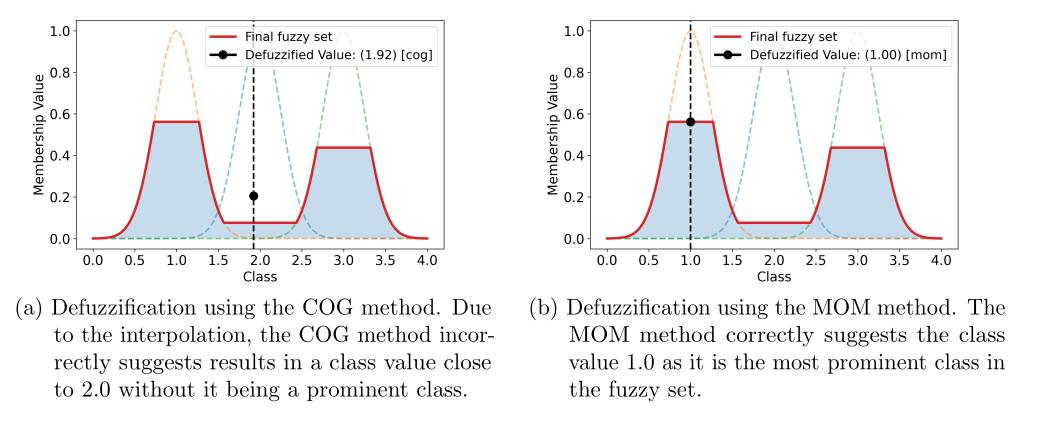
\includegraphics[width=0.7\textwidth, trim={1.2cm 4.8cm 2.9cm 0cm},clip]{figures/cog-vs-mom.png}
		
		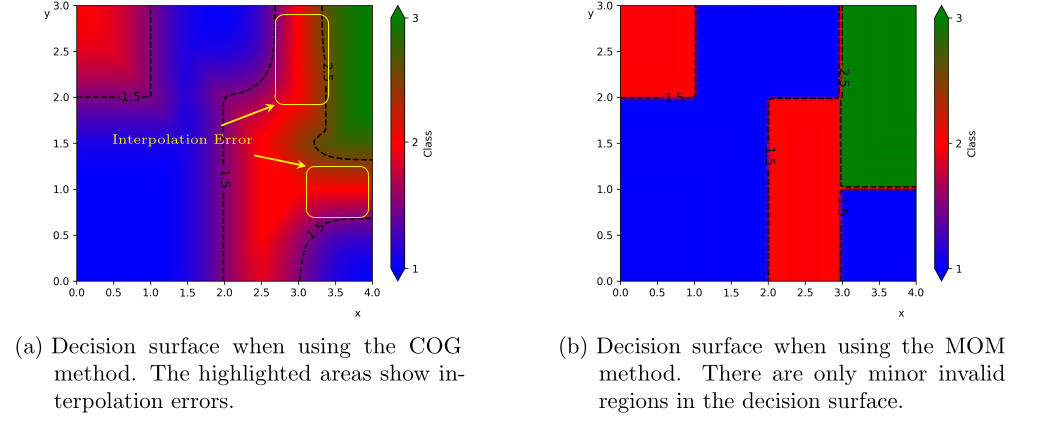
\includegraphics[width=0.78\textwidth, trim={0 3.7cm 2.3cm 0cm},clip]{figures/decision-surfaces.png}
	\end{figure}
	
\end{frame}

\begin{frame}
	\frametitle{Fuzzy Rule Extraction for \texttt{md\_flexible}}
	
	\begin{itemize}
		\item Collect dataset of \texttt{md\_flexible} simulations (FullSearch)
		\item For each tuning phase $i$, store:
		      \begin{itemize}
			      \item LiveInfoData: {\footnotesize \texttt{maxDensity, homogeneity, threadCount, \dots} }
			      \item TuningData: {\footnotesize \texttt{Container, Traversal, Newton3, \dots, \textbf{Time}} }
		      \end{itemize}
		\item Introduce \textit{relative speed} metric
		      \begin{itemize}
			      \item Absolute time is not meaningful across different \textit{environments}
			            \[ \text{relative speed}_{config}^{(i)} = \frac{\text{t}_{best}^{(i)}}{\text{t}_{\text{config}}^{(i)}} \]
		      \end{itemize}
	\end{itemize}
	
\end{frame}

\begin{frame}
	\frametitle{Resulting Dataset}
	
	\begin{itemize}
		\item Contains expected \textit{relative speed} based on:
		      \begin{itemize}
			      \item Simulation state
			      \item Configuration
		      \end{itemize}
		\item Forms basis for \textit{Suitability} and \textit{Component} tuning approaches
	\end{itemize}
	
	\begin{figure}
		\centering
		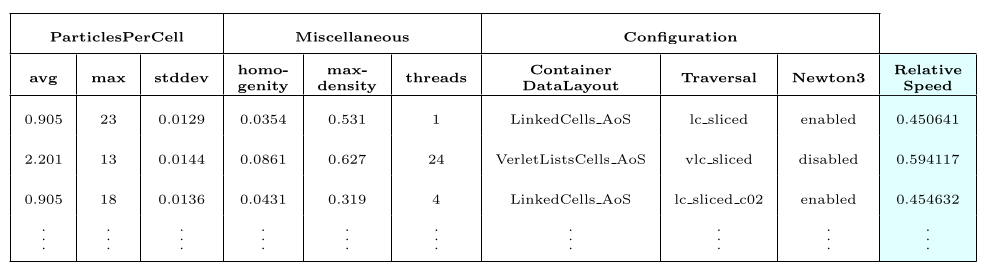
\includegraphics[width=1\textwidth]{figures/relative-speed-table.png}
	\end{figure}
	
\end{frame}

\begin{frame}
	\frametitle{Component Tuning: Extracted Rules}
	
	\begin{itemize}
		\item Preprocessing:
		      \begin{enumerate}
			      {\footnotesize
			      \item Naively remove bad configurations (relative speed $<70\%$)
			      \item Group remaining dataset by tuning-phase
			      \item Aggregate present (\textit{good}) values for each parameter
			            }
		      \end{enumerate}
		\item Apply Rule Extraction algorithm for each parameter
	\end{itemize}
	
	\begin{figure}
		\centering
		\vspace{-0.1cm}
		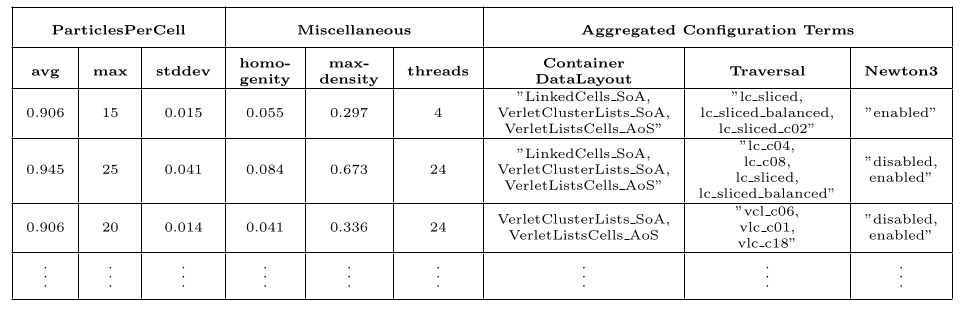
\includegraphics[width=0.93\textwidth, trim={0 3.8cm 0 0},clip]{figures/aggregated-data-component.png}
		\vspace{-0.1cm}
		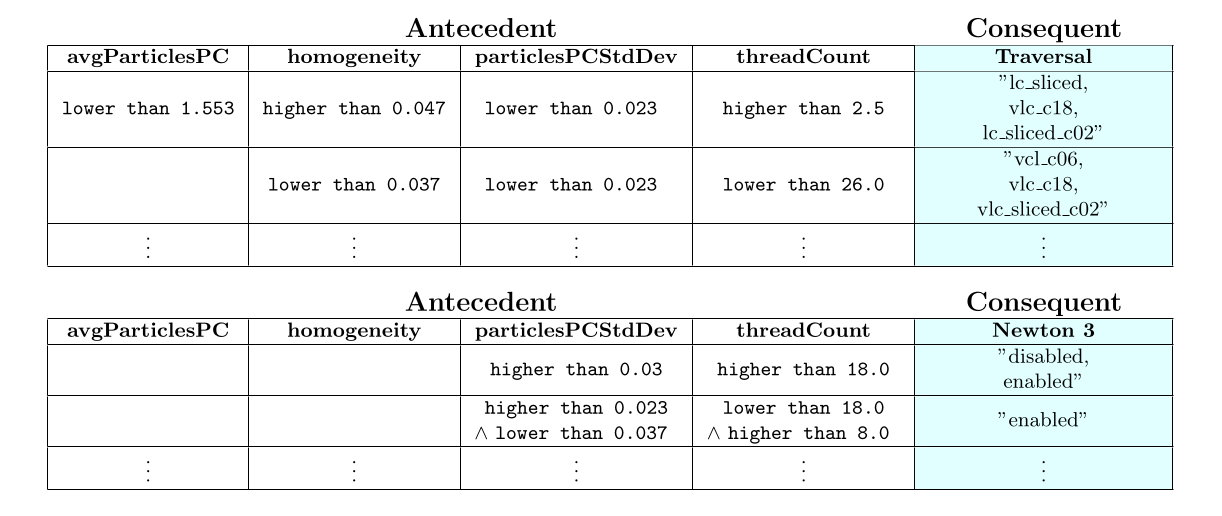
\includegraphics[width=0.98\textwidth, trim={0 8cm 0 0},clip]{figures/final-rules-component.png}
	\end{figure}
\end{frame}

\begin{frame}
	\frametitle{Suitability Tuning: Extracted Rules}
	
	\begin{itemize}
		\item Preprocessing:
		      \begin{enumerate}
			      {\footnotesize
			      \item Assign suitability-classes to each entry in the dataset
			            }
		      \end{enumerate}
		\item Extraction:
		      \begin{enumerate}
			      {\footnotesize
			      \item Group dataset by configuration
			      \item Apply Rule Extraction algorithm for each configuration
			            }
		      \end{enumerate}
	\end{itemize}
	
	\vspace{-0.1cm}
	
	\begin{figure}
		\centering
		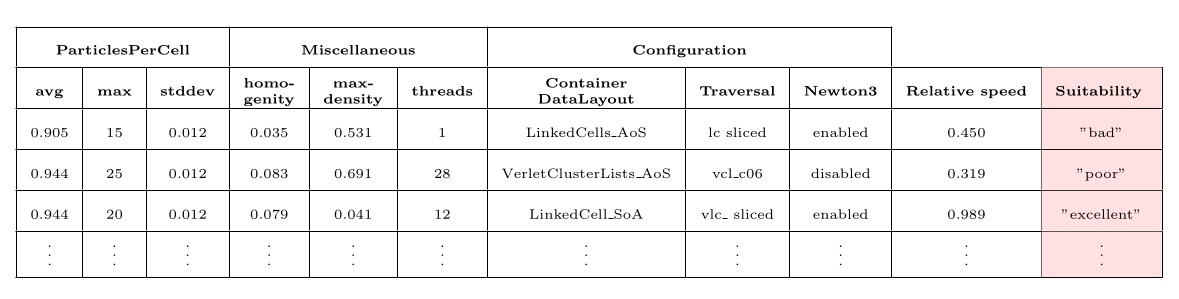
\includegraphics[width=1\textwidth, trim={0 2.25cm 0 0},clip]{figures/aggregated-data-suitability.png}
		\vspace{1.5cm}
		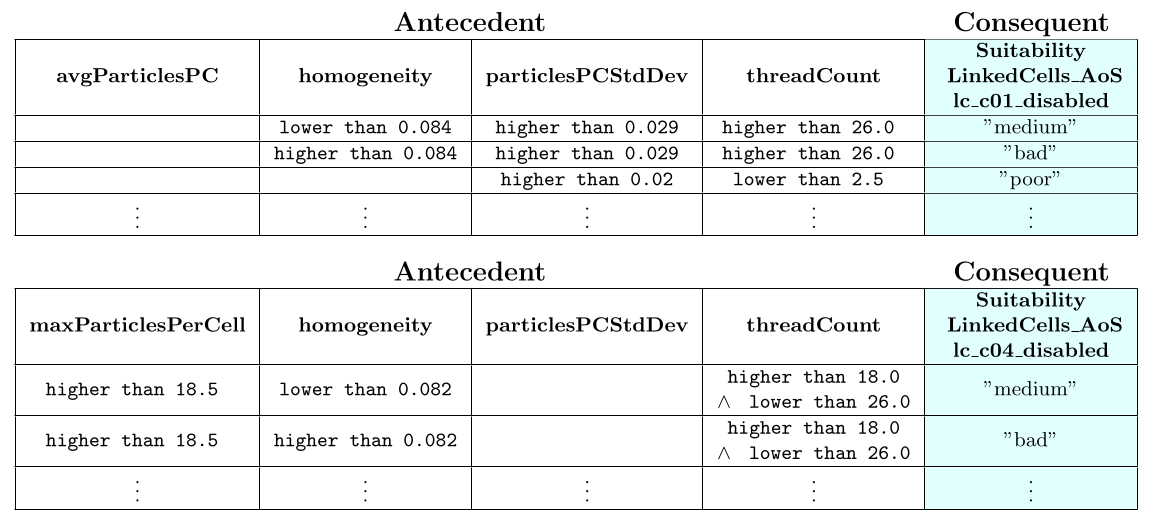
\includegraphics[width=1\textwidth, trim={0 9cm 0 0.1cm},clip]{figures/final-rules-suitability.png}
	\end{figure}
\end{frame}

\section{Benchmarks}
\begin{frame}
	\frametitle{Benchmark 1: Exploding Liquid}
	\begin{itemize}
		\item Exploding Liquid Benchmark (Included in Dataset)
		      \begin{itemize}
			      \item Both fuzzy approaches look promising
			      \item Very short tuning phases (not much noise)
			      \item Selected configurations perform well (tiny spikes)
			      \item Winning configurations are (mostly) equivalent
		      \end{itemize}
	\end{itemize}
	
	\begin{figure}
		\centering
		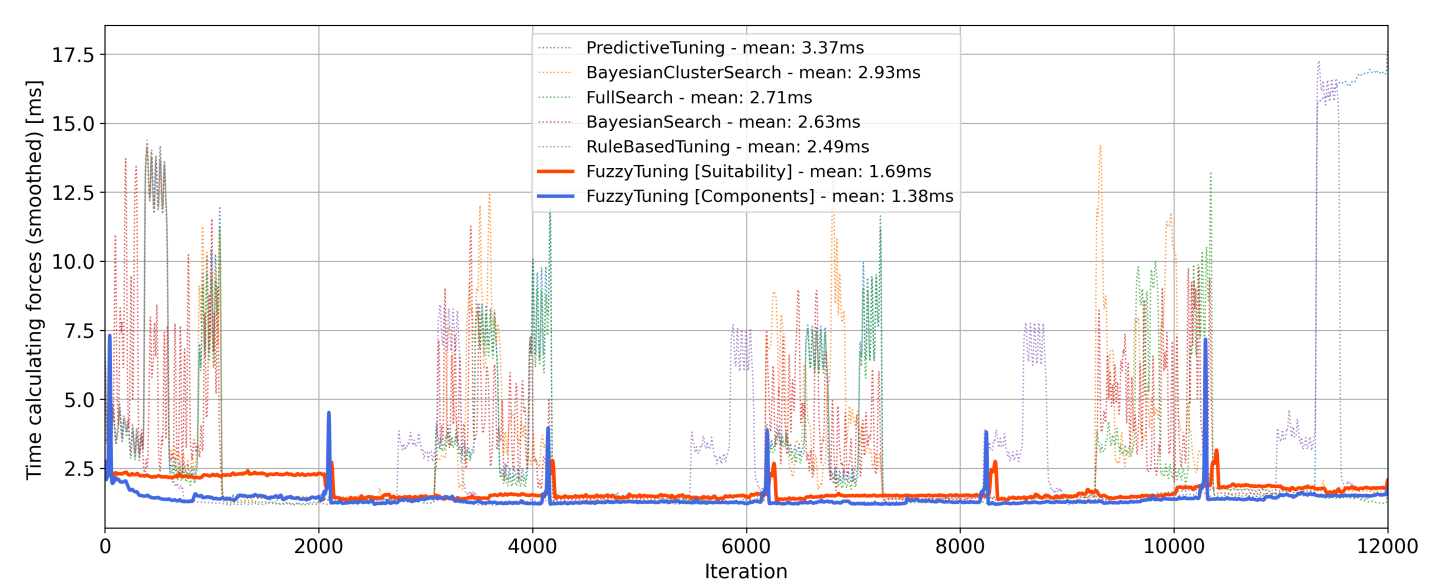
\includegraphics[width=1\textwidth]{figures/exploding-liquid-timings.png}
	\end{figure}
\end{frame}

\begin{frame}
	\frametitle{Total Time: Exploding Liquid}
	\begin{itemize}
		\item Fuzzy tuning has lowest total time
		\item Mostly due to the very efficient tuning phases:
		      \begin{itemize}
			      \item Few configurations evaluated
			      \item Evaluated configurations are expected to perform well
		      \end{itemize}
		\item Benefits of tuning with tiny tuning overhead
	\end{itemize}
	
	\begin{figure}
		\centering
		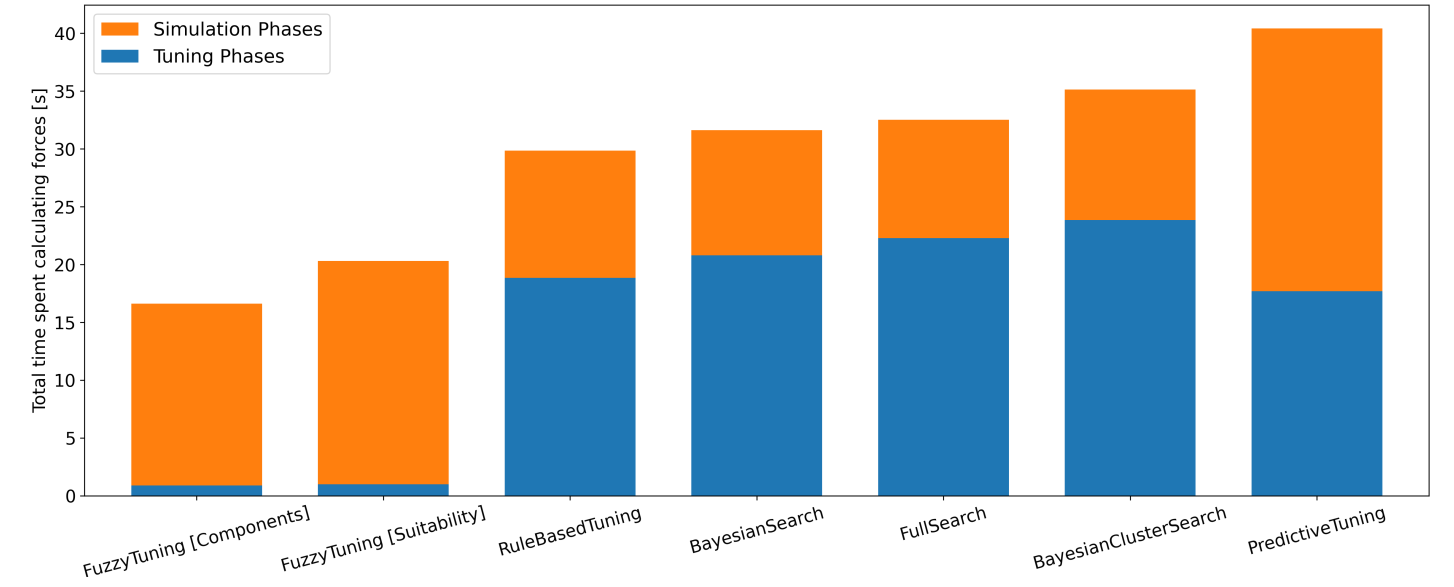
\includegraphics[width=0.95\textwidth]{figures/exploding-liquid-total.png}
	\end{figure}
\end{frame}

\begin{frame}
	\frametitle{Benchmark 2: Spinodal Decomposition MPI}
	
	\begin{itemize}
		\item Spinodal Decomposition MPI (Indirectly included in Dataset)
		      \begin{itemize}
			      \item Component approach performs well
			      \item Suitability approach struggles
			            \begin{itemize}
				            \item However, very fast tuning phases
				            \item Can this make up for the suboptimal configurations?
			            \end{itemize}
		      \end{itemize}
	\end{itemize}
	
	\vspace{-0.1cm}
	
	\begin{figure}
		\centering
		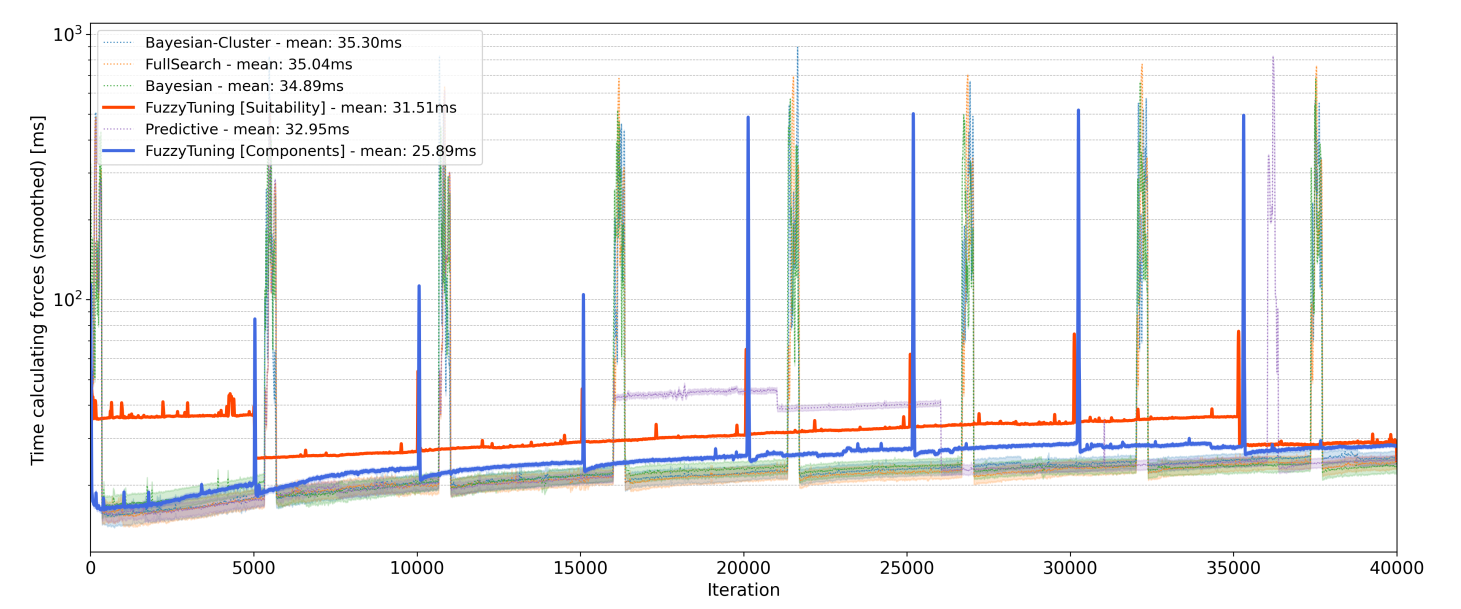
\includegraphics[width=1\textwidth]{figures/spinodal-timings.png}
	\end{figure}
\end{frame}

\begin{frame}
	\frametitle{Comparison and Evaluation: Spinodal Decomposition}
	
	\begin{itemize}
		\item Similar trends as previously
		\item Fast tuning phases compensate for suboptimal configurations!
		\item Improvements to the suitability approach:
		      \begin{itemize}
			      \item Increase suitability threshold $\rightarrow$ encourage longer tuning phases
			      \item Optimal: Evaluating Top 30\% {\scriptsize (instead of 10\%)} of configurations
		      \end{itemize}
	\end{itemize}
	
	\begin{figure}
		\centering
		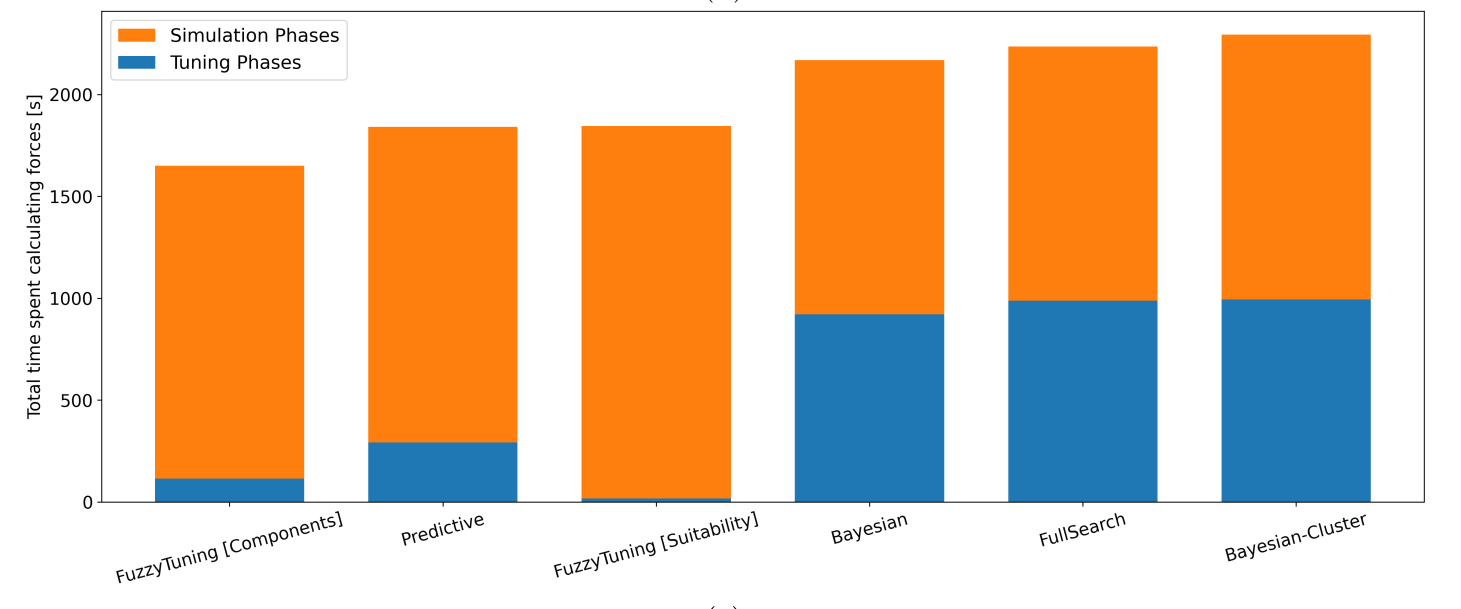
\includegraphics[width=0.92\textwidth]{figures/spinodal-total.png}
	\end{figure}
\end{frame}


\section{Conclusion}

\begin{frame}
	\frametitle{Conclusion}
	\begin{itemize}
		\item Fuzzy Logic is very promising for tuning AutoPas
		      \begin{itemize}
			      \item Massive reduction in tuning overhead
			      \item Still competitive results
		      \end{itemize}
		\item Data-Driven Rule Extraction is a good starting point
		      \begin{itemize}
			      \item \textbf{Benefits:}\\
			            \quad \cmark \; No need for expert knowledge\\
			            \quad \cmark \; Semi-automated process\\
			            \quad \cmark \; Generalizes to new applications\\
			            \quad \cmark \; Interpretabilty is a huge benefit
			      \item \textbf{Drawbacks:}\\
			            \quad \xmark \; Requires a lot of data (1.1GB) \\
			            \quad \xmark \; Unapealing for users \\
			            \quad \xmark \; Maybe too complex for simple problems
		      \end{itemize}
		      
	\end{itemize}
\end{frame}


\begin{frame}
	\frametitle{Future Work}
	\begin{itemize}
		\item Dynamic Rule Generation
		      \begin{itemize}
			      \item Update expert knowledge on the fly
			      \item No need for giant datasets
			      \item Could automatically adapt to new scenarios / applications
		      \end{itemize}
		\item General Improvements to the Tuning Process
		      \begin{itemize}
			      \item Investigate early stopping mechanism
			      \item Stop evaluating extremely bad configurations early
			      \item Maybe solve the tuning overhead once and for all
		      \end{itemize}
		\item Simplification of the Model
		      \begin{itemize}
			      \item Decision Trees instead of Fuzzy Systems
			      \item Easier to maintain and understand
			      \item Maybe comparable results
		      \end{itemize}
	\end{itemize}
\end{frame}


\begin{frame}
	\begin{center}
		\vspace{1cm}
		{\large \textbf{Thank you for your attention!}}
		
		\vspace{2cm}
		
		\Huge{Questions?}
	\end{center}
\end{frame}

\thispagestyle{empty}
\begin{frame}[allowframebreaks, noframenumbering]
	\frametitle{References}
	\footnotesize
	\bibliographystyle{apalike}
	\bibliography{literature}
\end{frame}

\end{document}
